%!TEX root = ../main.tex
\setcounter{page}{0}
\thispagestyle{fancy-blank}
\begingroup
% \vphantom{Optional note}
{\large \par}
\vspace*{35mm}
{\huge\bfseries\utitle\par}

\vspace*{4mm}
{\rule{\linewidth}{0.5mm}\par}
\vspace*{4mm}

{\large\bfseries\uauthor\par}\vspace*{1mm}

{\large\itshape{a kolektiv}\par}


\vspace{10em}
\begin{figure}[ht!]
\begin{center}
  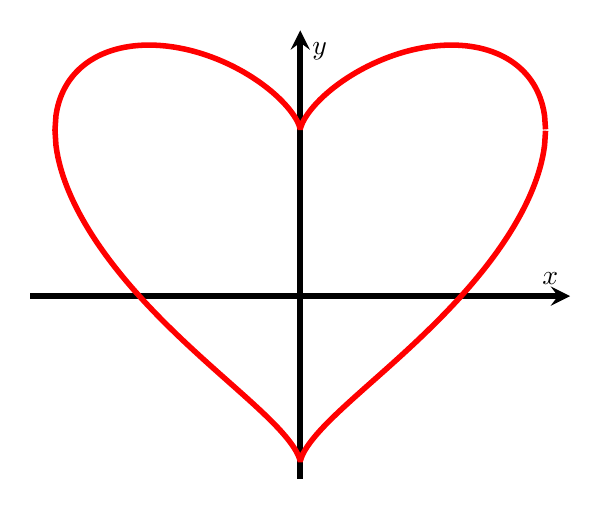
\begin{tikzpicture}
  \begin{axis}[
      axis lines = middle,
      xlabel = \(x\),
      ylabel = {\(y\)},
      xmin=-1.1,
      xmax=1.1,
      ymin=-1.1,
      ymax=1.6,
      xtick = \empty,
      ytick = \empty,
      line width=2pt,
  ]
  %Below the red parabola is defined
  \addplot [
      domain=-1:1,
      samples=500,
      color=red,
  ]
  {abs(x)^(2/3)+sqrt(1 - x^2)};

  \addplot [
      domain=-1:1,
      samples=500,
      color=red,
      ]
      {abs(x)^(2/3)-sqrt(1 - x^2)};

  \end{axis}
  \end{tikzpicture}
  \caption*{Graf $x^2+ \left [ y- x^\frac{2}{3} \right ]^2 = 1$}
\end{center}
\end{figure}
\vfill
{\large \par}
\endgroup
\clearpage
